

\chapter{\datalogra on Spark}\label{r:implementation}

\datalogra queries executed in a distributed way can prove to be very useful for performing computations on large datasets, especially on graphs. Our goal is to provide an implementation of \datalogra which will be as close as possible to being practically applicable.

To be truly useful, such solution has to be reliable, provide ways to interact with various distributed storages, ensure proper fault tolerance and require little to no additional work to be run on the existing infrastructure.

Distributed Socialite, covered in section \ref{s:distributed}, executes queries with aggregation in a distributed way by sharding the data based on a selected column of each relation. Its authors presented an independent implementation of the proposed solution. We propose an alternative approach to distributed \datalogra queries evaluation and present an implementation of the proposed solution.

Instead of developing an independent project, we have chosen to implement \datalogra as an extension to Apache Spark. Owing to this approach, the implementation can read from and write to all popular Hadoop distributed data stores, including HDFS, HBase and Cassandra \cite{sparkwww}. It can be used on any existing cluster that supports Spark, including Hadoop YARN \cite{hadoop}, Mesos and standalone Spark clusters \cite{sparkwww} and has the industrial-quality fault tolerance and efficiency features developed by hundreds of Apache Spark contributors \cite{githubspark}. 

Using Spark Datalog API, \datalogra queries can be integrated seamlessly into Spark programs. One can choose to use Datalog for all computations or only for their parts where it serves best. It is also possible to run \datalogra queries interactively using the Spark Shell.

In this chapter we describe how Datalog and \datalogra queries can be translated into operations permitted in the RDD model. This method was used to implement the Datalog API for Spark, allowing for the usage of Datalog queries in Spark programs. The implementation is evaluated in section \ref{s:impl_eval}.

\section{Integrating \datalogra into Spark}

Spark programs describe the computation as a series of calls to functions which perform one of the following:
\begin{itemize}
  \item create an RDD, generally by reading it from a distributed data source such as HDFS,
  \item transform an RDD or several RDDs into another RDD with methods such as \emph{map}, \emph{filter} or \emph{join},
  \item execute an action on an RDD, such as storing it in HDFS or counting its size.
\end{itemize}

Most of the computation logic is expressed with transformations.  Core Spark provides only some basic transformations (such as \emph{map, filter, reduceByKey, union, join, sample, sort}) and actions (e.g. \emph{count, collect, reduce, save}). Additionally, there are several extensions: GraphX, Spark SQL, MLlib. Typically, they extend Spark by providing specialized RDDs and composite data structures as well as additional transformations for them.

The same approach has been chosen for adding the ability to execute Datalog queries. The extension is contained in a module called \emph{Spark Datalog API} or \emph{SparkDatalog}. The main component it provides is the \emph{Database} class which contains a set of relations and can be created from regular RDDs. Database objects are equipped with a method \emph{datalog}, which performs a Datalog query on this database. The result of the query is a new Database, from which individual relations can be extracted as RDDs. 

Datalog queries can be applied to any set of input RDDs. The input data can be directly loaded from a distributed storage supported by Spark or computed as a transformation of other RDDs. The user first creates relations, declares their arity, and groups them into a database. Next, any query on this database can be performed using its \emph{datalog} method. If there are no errors in the query, the result is a new database containing all computed relations. Each relation can be extracted from the database by giving its name. Figure \ref{sdinspark} shows an example of a \datalogra query in a Spark program using Datalog API for Spark.

\begin{figure}[!htbp]
  \centering
\begin{Verbatim}
\textcolor{RedViolet}{val} \textcolor{RoyalPurple}{edgesRdd} = \textcolor{gray}{... // RDD of edge tuples read from disk or computed using Spark}

\textcolor{RedViolet}{val} \textcolor{RoyalPurple}{database} = \textcolor{RoyalPurple}{Database}(\textcolor{RoyalPurple}{Relation}.ternary(\textcolor{BurntOrange}{"Edge"}, edgesRdd))
\textcolor{RedViolet}{val} \textcolor{RoyalPurple}{resultDatabase} = database.datalog(\textcolor{vdarkgray}{"""}
    \textcolor{vdarkgray}{\textcolor{RedViolet}{declare} \textcolor{RoyalPurple}{Path}(int v, int dist \textcolor{RedViolet}{aggregate} Min).}
    \textcolor{vdarkgray}{\textcolor{RoyalPurple}{Path}(x, d) :- s == 1, \textcolor{RoyalPurple}{Edge}(s, x, d).}
    \textcolor{vdarkgray}{\textcolor{RoyalPurple}{Path}(x, d) :- \textcolor{RoyalPurple}{Path}(y, da), \textcolor{RoyalPurple}{Edge}(y, x, db), d = da + db.}
\textcolor{vdarkgray}{"""})
\textcolor{RedViolet}{val} \textcolor{RoyalPurple}{resultPathsRdd} = resultDatabase(\textcolor{BurntOrange}{"Path"})

\textcolor{gray}{... // Save or use resultPathsRdd as any RDD.}
\end{Verbatim}
  \caption{Example of Datalog query for computing single source shortest paths embedded in a Spark program.\label{sdinspark}}
\end{figure}
\section{Executing \datalogra queries in the RDD model}

When a Datalog query is performed on the Database object, it needs to be translated into a sequence of Spark transformations which eventually produce a new Database object containing the result of the query. In this section, we show how this translation is made.

\subsection{Data representation}

Both input and output of Datalog programs are represented as Database objects. Database is simply a set of several Relations.

Each Relation object has a name and an RDD of Facts, which in turn are represented as arrays. All Facts in a relation are required to have the same arity --- this is ensured when the Relation is created.

\emph{Valuation} objects are not available to the end user, but they play a significant role in the evaluation. They represent valuations, i.e. functions mapping variables to their values. For performance reasons, they are not represented as maps, but as raw arrays whose layout is determined using the information generated during the analysis phase.

\subsection{Datalog program execution}

On the top level, the algorithm for executing a Datalog program on Spark consists of the following steps:

\begin{enumerate}
\item Analysis phase: Initially, the program is parsed and analyzed both syntactically and semantically. All correctness requirements are checked at this stage.

\item Stratification: Analyzed program is then stratified, i.e. divided into a sequence of strata using a standard strongly connected components algorithm.

\item Evaluation phase, which starts by evaluating the first stratum of the program on the input database. Each subsequent stratum is then evaluated using the output of the previous stratum as an input. The output of the last stratum is returned as the output of the whole program.

\end{enumerate}

To evaluate each stratum, the semi-naive evaluation algorithm is used. It maintains the current state of the database and runs iteratively until no changes are made to the database. In each iteration, for each rule in this stratum, all inferable facts are computed. The way this can be achieved on RDDs is described in section \ref{ss:impl_evalrule}. The set of obtained facts is then merged into the current database and a \emph{delta}, i.e. the difference between the current and previous database state is computed. During the merge all necessary aggregations are applied. This step is described in Section \ref{ss:impl_merge}.

\subsection{Single rule evaluation}\label{ss:impl_evalrule}
Evaluation of a single rule plays a crucial role in evaluating a Datalog query on RDDs. Given a single rule, consisting of a head and a sequence of subgoals, and two databases: the full database state after the last step and the delta database, the task is to compute an RDD of all facts that can be inferred. It is done in two steps: first, all valuations satisfying the rule body are computed, and then each such valuation is converted to a fact based on the head of the rule.

The subgoals are sorted topologically during the analysis phase, so that the evaluation can be performed sequentially, subgoal by subgoal. We keep the RDD of all valuations which satisfy the subgoals processed so far. This RDD is updated in each step. The topological order ensures that all variables required by arithmetic subgoals are introduced by an earlier subgoal. 

We start with an RDD of valuations containing an empty valuation, i.e. a valuation containing no variable assignments. Next, the subgoals are applied sequentially. Each subgoal is evaluated on the current RDD of valuations. This returns a new RDD of valuations all of which satisfy this subgoal. This new RDD is then used for the next subgoal, until all subgoals are processed.

Before describing how a subgoal is evaluated on an RDD of valuations, we first describe a simplified scenario of processing a subgoal given a single valuation. Then we show how generated valuations are converted into facts and how these general methods can be used to perform either naive or semi-naive evaluation. Finally, we describe how new facts are merged into the existing database.

\subsubsection{Evaluating a subgoal on a single valuation}
Let us start from the most basic scenario. Let us assume that we already have some valuation $v$ to start with. $v$ simply defines a specific value for some variables. The task is to evaluate a single relational subgoal $R(x_1, \dots, x_n)$ on the starting valuation $v$, i.e. to find the set of all valuations which satisfy $R(x_1, \dots, x_n)$ and are supersets of $v$. To do this, we can find all facts in relation $R$ that match $v$ on the \emph{matching variables}, i.e. those which appear both in the valuation and in the subgoal. Each such fact yields an extended valuation consisting of $v$ and the valuation for variables from the subgoal. 

For example, given a subgoal \relat{Edge}{(v, u, d)} and a valuation $\{v: 5, t: 3\}$, if \textsc{Edge}  contains \relat{Edge}{(5, 1, 2)}, \relat{Edge}{(5, 3, 4)} and \relat{Edge}{(1, 2, 3)}, the result will be $\{\{v: 5, t: 3, u: 1, d: 2\}, \{v: 5, t: 3, u: 3, d: 4\}\}$.

This algorithm could be realized by means of \emph{map} and \emph{filter} transformations on the relation in the subgoal.

Other types of subgoals are more straightforward. Arithmetic comparison subgoals, e.g. $x < y + z$ are simply evaluated to a boolean value and yield $\{v\}$ if the result was true, and an empty set if the result was not true. In case of assignment subgoals, e.g. $x = y + z$, the value of the expression is calculated inserted into the valuation for the given variable. If this causes a conflict with a different value for that variable, an empty set is returned. Otherwise, the result is a singleton containing the new variable.

\subsubsection{Evaluating a subgoal on a set of valuations}
During the evaluation of a sequence of subgoals, instead of having just one starting valuation, we have an RDD of valuations to start with. The result of evaluating a subgoal on an RDD of valuations should be an RDD with all valuations satisfying the subgoal and being supersets of at least one of the starting valuations.

In case of relational subgoals, to find the result efficiently, the relation is first converted into valuations of variables in the subgoal using a \emph{map} transformation. The resulting RDD is then joined with the starting valuations on the matching variables using the \emph{join} transformation on RDDs and mapped to a new RDD of valuations. This is illustrated in Figure \ref{graphevalrelsubgoalrddval}.

\tikzstyle{rect} = [rectangle, minimum width=2.5cm, minimum height=1cm,text centered, draw=black, align=left]
\tikzstyle{arrow} = [thick,->,>=stealth]
\tikzstyle{label} = [font=\scriptsize]

\begin{figure}[!ht]
\centering
\begin{tikzpicture}[node distance=2cm]

\node (start) [rect] {\relat{Rel}{(7, 1)}\\\relat{Rel}{(8, 1)}\\\relat{Rel}{(9, 2)}};

\node (mapped) [rect, below of = start, yshift=-1cm] {$\{x: 1, z: 7\}$\\$\{x: 1, z: 8\}$\\$\{x: 2, z: 9\}$};

\node (input) [rect, below of = mapped, xshift = -4cm] {$\{x: 1, y: 3\}$\\$\{x: 3, y: 5\}$};


\node (output) [rect, below of = mapped, xshift = 6cm] {$\{x: 1, y: 3, z: 7\}$\\$\{x: 1, y: 3, z: 8\}$};

\node (labelinput) [label, above of = input, yshift=-1cm] {starting valuations RDD};

\node (labeloutput) [label, above of = output, yshift=-1cm] {resulting valuations RDD};

\node (labelstart) [label, above of = start, yshift=-0.8cm] {facts in relation};

\node (join) [below of = mapped, yshift=-0.12cm] {};

\draw [arrow] (start) -- node[anchor=west] {\emph{map} using \relat{Rel}{(z, x)}} (mapped);

\draw[-] (mapped) -- (join);
\draw[arrow] (input) -- node[anchor=south, xshift=1.5cm] {\emph{join} and \emph{map}} (output);

\end{tikzpicture}
\caption{Evaluation of a relational subgoal \relat{Rel}{(z, x)} on an RDD of valuations.}\label{graphevalrelsubgoalrddval}
\end{figure}

Arithmetic comparison subgoals are translated into a \emph{filter} transformation on the valuations RDD. They are filtered using a function that checks whether the comparison yields true for that valuation. This is illustrated in Figure \ref{graphevalarithmsubgoalrddval}. 


\begin{figure}[!ht]
\centering
\begin{tikzpicture}[node distance=2cm]

\node (input) [rect, xshift = -4cm] {$\{x: 1, y: 2, z: 5\}$\\$\{x: 1, y: 2, z: 2\}$};

\node (output) [rect, xshift = 6cm] {$\{x: 1, y: 2, z: 5\}$};

\node (labelinput) [label, above of = input, yshift=-1cm] {starting valuations RDD};

\node (labeloutput) [label, above of = output, yshift=-1cm] {resulting valuations RDD};

\draw[arrow] (input) -- node[anchor=south] {\emph{filter} by $z > x + y$} (output);

\end{tikzpicture}
\caption{Evaluation of an arithmetic comparison subgoal $z > x + y$ on an RDD of valuations.}\label{graphevalarithmsubgoalrddval}
\end{figure}


Assignment subgoals are translated into a \emph{map} transformation on the valuations RDD, combined with flattening of the results. For each valuation, the assignment can be mapped either to a singleton or to an empty set, so the result of applying the mapping is an RDD of sets. Therefore it needs to be flattened so that the result is a plain RDD of valuations. Figure \ref{graphevalassignsubgoalrddval} illustrates these two steps.


\begin{figure}[!ht]
\centering
\begin{tikzpicture}[node distance=2cm]

\node (input) [rect, xshift = -5cm] {$\{x: 1, y: 2\}$\\$\{y: 3\}$};

\node (middle) [rect] {$\{\emptyset\}$\\$\{\{{x: 6, y: 3}\}\}$};

\node (output) [rect, xshift = 5cm] {$\{x: 6, y: 3\}$};

\node (labelinput) [label, above of = input, yshift=-1cm] {starting valuations RDD};

\node (labeloutput) [label, above of = output, yshift=-1cm] {resulting valuations RDD};

\draw[arrow] (input) -- node[anchor=south] {\emph{map}} (middle);

\draw[arrow] (middle) -- node[anchor=south] {\emph{flatten}} (output);

\end{tikzpicture}
\caption{Evaluation of an assignment subgoal $x = 2 * y$ on an RDD of valuations.}\label{graphevalassignsubgoalrddval}
\end{figure}


\subsubsection{Processing rule head: converting valuations into facts}

Each rule head consists of a relation name and a sequence of variable names, e.g. \relat{Path}{(v, d)}. Language constraints ensure that each valuation satisfying the rule body contains values for all variables appearing in the head, so a fact can be computed from a valuation by looking up corresponding variables in the valuation. Given an RDD of valuations obtained by evaluating the sequence of subgoals in the rule body, this is done by applying a \emph{map} transformation to this RDD. This is illustrated in Figure \ref{graphevalrulehead}.


\begin{figure}[!ht]
\centering
\begin{tikzpicture}[node distance=2cm]

\node (start) [rect] {$\{x: 1, y: 3, z: 7\}$\\$\{x: 1, y: 5, z: 8\}$};

\node (output) [rect, right of = start, xshift = 8cm] {\relat{Rel}{(7, 1)}\\\relat{Rel}{(8, 1)}};

\node (labeloutput) [label, above of = output, yshift=-1cm] {RDD of facts};

\node (labelstart) [label, above of = start, yshift=-1cm] {valuations RDD};

\draw[arrow] (start) -- node[anchor=south] {\emph{map} using \relat{Rel}{(z, x)}} (output);

\end{tikzpicture}
\caption{Converting valuations into facts based on the rule head.}\label{graphevalrulehead}
\end{figure}

\subsubsection{Naive and semi-naive evaluation}
If full database is used to retrieve the contents of the relation in each subgoal, the evaluation procedure described in the previous sections will perform the naive evaluation.

For the semi-naive evaluation to be performed, the delta database needs to be used. Precisely, the rule body is evaluated separately for each subgoal that uses a relation being in the \emph{idb} of the current stratum. The contents of the relation for the selected subgoal is retrieved from the delta database and the full database is used in all other subgoals.

\subsection{Adding new facts to the database}\label{ss:impl_merge}

The procedure covered in section \ref{ss:impl_evalrule} allows for finding all facts that can be inferred using a single rule. This can be done for each rule within a stratum. The next step in one iteration of evaluation is to merge the results obtained with the existing database.

In case of relations without aggregation, this is achieved by performing the \emph{union} transformation on the RDDs containing new facts for a given relation and the corresponding relation in the current database. It is possible that this introduces duplicated facts, so the \emph{distinct} transformation is used to remove the duplicates.

In case of relations that need to be aggregated, this is slightly different. After performing a union of the new facts and current relation contents, the facts are grouped by the qualifying parameters and the aggregated value is computed by applying the aggregation function. This is done by performing the following three transformations:
\begin{enumerate}
\item \emph{map} to split the facts into qualifying parameters and the aggregated values,
\item \emph{reduceByKey} to group by qualifying parameters and apply the aggregation function to the set of aggregated values in each group,
\item \emph{map} to merge the qualifying parameters and the computed value in each group back into facts.
\end{enumerate}
This process is illustrated in Figure \ref{graphaggregate}.


\begin{figure}[!ht]
\centering
\begin{tikzpicture}[node distance=4cm]

\node (input) [rect] {$(1, 2, 5)$\\$(1, 2, 7$)\\$(1, 3, 9)$\\$(1, 3, 4)$};

\node (split) [rect, right of=input] {$(1, 2) \to 5$\\$(1, 2) \to 7$\\$(1, 3) \to 9$\\$(1, 3) \to 4$};

\node (reduced) [rect, below of=split, yshift=0.5cm] {$(1, 2) \to 5$\\$(1, 3) \to 4$};

\node (merged) [rect, left of=reduced] {$(1, 2, 5)$\\$(1, 3, 4)$};

\node (labelinput) [label, above of = input, yshift=-2.52cm] {RDD of unaggregated facts};

\node (labeloutput) [label, above of = merged, yshift=-3cm] {aggregated facts RDD};

\draw[arrow] (input) -- node[anchor=south] {\emph{map}} (split);
\draw[arrow] (split) -- node[anchor=west] {\emph{reduceByKey} with \emph{min}} (reduced);
\draw[arrow] (reduced) -- node[anchor=south] {\emph{map}} (merged);

\end{tikzpicture}
\caption{Applying \emph{min} aggregation to third column of an RDD of facts.}\label{graphaggregate}
\end{figure}


\subsection{Handling RDD caching, materialization and lineage}
A practical implementation of the evaluation procedure described above requires several RDD-specific issues to be handled:
\begin{itemize}
\item reused RDDs need to be marked to be \emph{cached} in order for them to be stored in memory and not recomputed each time they are used. The new full database and delta database are marked for caching after each iteration step,
\item results obtained from an iteration and marked to be cached are materialized, i.e. actually computed. This allows for the results of the previous iteration to be \emph{unpersisted}, i.e. removed from cache, as they will no longer be necessary. In each step, after the full database and delta are materialized, their older versions are unpersisted. Unpersisting RDDs helps reduce memory usage and increases performance,
\item if many iterations are performed, the procedure can create RDDs with a very long \emph{lineage}. Lineage is stored in RDDs so that they can be restored after a failure of a worker. Too long lineage can cause errors, so every several iterations all results are checkpointed to persistent storage, which causes the lineage to be cropped,
\item most of RDD transformations do not change the partitioning of data, i.e. the way the data is distributed between worker nodes. However, \emph{join} transformations, which are used in the evaluation, increase the number of partitions. The number of partitions too large compared to the size of data can negatively affect performance, so it is reduced when it exceeds a certain limit using the \emph{coalesce} action, which merges certain partitions of an RDD to reduce their number. Currently, the limit is defined manually, but it could be possibly computed based on the amount of data and the number of worker nodes. 
\end{itemize}


\subsection{Optimizations}
The main implemented optimization was the semi-naive evaluation. Additionally, several smaller optimizations have been implemented:
\begin{itemize}
\item Usually some of the strata are non-recursive and define only one relation. In this case, it is clear upfront that one iteration is enough for all facts to be inferred, so the evaluation of the stratum is finished after one iteration, instead of performing one more iteration only to notice that there were no changes in the database.
\item Rule bodies can start with constant subgoals, e.g. $\textsc{Path}(v,t) :-~s=1, \textsc{Edge}(s, v, t)$. When subgoals are topologically sorted, such subgoals are placed at the beginning of the subgoals sequence. In order for the evaluation of the constant subgoals not to be repeated, the initial sequence of constant subgoals is evaluated during the analysis phase. The result is then used as an initial valuation when evaluating the rest of the subgoals in each iteration where this rule body is considered.
\item If a relation is used in a subgoal, it needs to be converted into an RDD of valuations for joins to be performed. From the perspective of a stratum, however, only the relations defined in this particular stratum can change. Therefore, within each stratum, for each subgoal referring to a relation from another stratum the corresponding valuations are found once and persisted. It makes it possible to avoid repeated work in each of the evaluation iterations in this stratum.
\end{itemize}

\section{Experiments}\label{s:impl_eval}
Spark Datalog API has been implemented as a fully working prototype. It has been evaluated on clusters of up to 16 Amazon EC2 worker instances. In this section we provide three sets of experimental results. \datalogra is not limited to a specific domain and can be used to express various types of distributed computations, but it is primarily intended for computations on large graphs such as social networks. Therefore, we have selected three common graph problems \cite{ullman, pregel} for performance tests of the prototype implementation:
\begin{itemize}
\item finding and counting triangles: find all triangles in a graph, i.e. triplets of vertices which form a complete graph; additionally, the total count of triangles should be computed,
\item dividing the graph into connected components, i.e. maximal subgraphs in which each pair of vertices is connected by a path,
\item computing the shortest paths from a single source to all other vertices.
\end{itemize}

The performance of the tested implementation was compared with plain Spark programs solving the same problem. The plain Spark implementations were written using Spark core methods and the \emph{pregel} operation provided by the GraphX extension. In addition to performance, an interesting property is the complexity of each solution, which can be roughly measured by the number of lines in each program. To our knowledge, only an implementation of a sequential version of SociaLite was publicly available at the time of our tests. In the future, a comparison with Distributed Socialite will also be interesting.

For each problem, both solutions have been evaluated on Amazon EC2 clusters consisting of $n = 2, 4, 8$ and $16$ worker nodes and one master node. Each node was a 2-core 64-bit machine with 7.5 GiB of RAM memory.  In all experiments, a social graph of Twitter circles \cite{twitterdata}, which has 2.4M edges was used.

For both SparkDatalog and plain Spark programs the execution times $T_n$ were measured in each test case, where $n$ is the number of worker nodes. Relative speedups, i.e. the ratio of $T_n$ to $T_2$ were calculated. Figure \ref{img_plots_exp} presents the execution times and the relative speedups compared to the ideal speedup. In the Triangles Count test case the execution time in SparkDatalog is very similar to dedicated Spark. The SparkDatalog versions are slower than dedicated Spark programs in both Shortest Paths and Connected Components, by a factor of approximately 8.5 to 3.5 in Shortest Paths and 4 - 1.7 in Connected Components. The reasons for that are analyzed in section \ref{s:whyslow}. The speedups achieved were similar for both versions of each program. This shows that although the implemented solution is slower by some factor, it does parallelize. The speedups were slightly better for the SparkDatalog versions. This is probably because of the fact that the additional overhead in SparkDatalog execution time over dedicated Spark could also get parallelized. In Connected Components and Shortest Paths, the difference in execution times is the least with the greatest number of worker nodes.

\begin{figure}[!htbp]
  \centering
    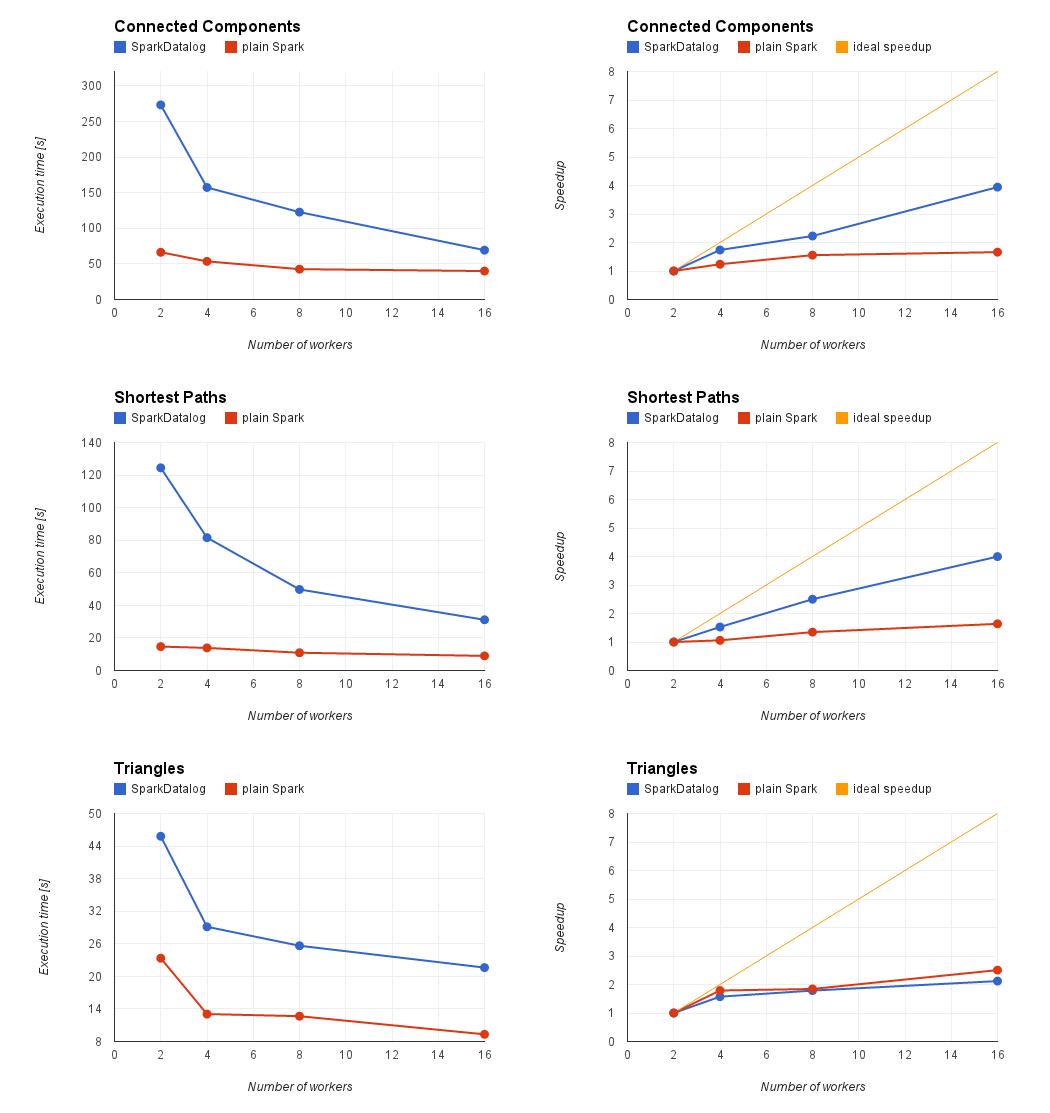
\includegraphics[width=\textwidth]{images/plots_all.png}
   \caption{Results of experiments. \label{img_plots_exp}}
\end{figure}


\begin{table}[!htbp]
  \centering
\begin{tabular}{|l|r|r|}
\hline   & \textbf{plain Spark} & \textbf{SparkDatalog} \\ 
\hline
 \textit{Connected Components} & 11 & 6 \\ 
 \textit{Shortest Paths} & 12 & 4 \\ 
 \textit{Triangles} & 7 & 5 \\ 
\hline 
\end{tabular} 
\caption{Number of lines of code in programs, excluding data loading and comments.}
\label{tab_proglen}
\end{table}

An important goal for SparkDatalog is to provide programmers and non-programming analysts with the possibility to perform computations by writing declarative queries instead of implementing complicated, lengthy algorithms using the Pregel model or standard RDD transformations. Table \ref{tab_proglen} shows the comparison of lengths between SparkDatalog and plain Spark programs for each of the problems. Datalog versions are 1.4 to 3.5 shorter than dedicated Spark. Most importantly, they are conceptually simpler since they only require a few declarative rules instead of expressing the problem in the vertex-centric Pregel model.

The source codes of programs used in the experiments are presented in Appendix \ref{appendixa}.

\section{Performance differences}\label{s:whyslow}
The SparkDatalog programs are several times slower than their dedicated Spark counterparts. There are several reasons for that, which can be eliminated or minimized in future versions of SparkDatalog:
\begin{enumerate}
\item SparkDatalog uses a general way of converting the Datalog program to a sequence of Spark transformations, which results in a suboptimal execution of the query, whereas the dedicated Spark program executes precisely the necessary operations. This can be resolved or minimized by more work on optimizing the generated execution plan.
\item The internal data representation has a significant impact on the performance. In dedicated Spark programs, native Scala tuples are used. SparkDatalog, on the other hand, currently uses arrays, which are less efficiently serialized and hashed. This results in a significant performance overhead. This could be resolved by representing the most common arities, e.g. 1--20 with tuples and using pre-generated code to work with them.
\item The most costly operation in SparkDatalog execution is the repartitioning of the objects by the hash of their key in order to perform a \emph{join}. The partitioning of the data could be optimized, so that the need to transfer and repartition the data is minimized. This can possibly result in a significant performance gain.
\end{enumerate}

In addition to the above, it is worth adding that since in Datalog problems are expressed in a very high-level, declarative way it offers large possibilities of applying optimizations to query execution, for example the \emph{delta-stepping} technique and approximate evaluation \cite{distsoc}. This can result in significant performance gains over plain Spark programs.

\section{Further work}

There are several areas for further work connected both to the implementation and to the proposed theoretical solution.

Currently, it is the user's responsibility to ensure that the program is correct and, in particular, that the rules are monotone with respect to the order implied by the aggregation function used. A theoretical result or an implementation of a tool helping to determine whether a program satisfies this condition is crucial for the wide adoption of the proposed language.

Clearly, the performance of the solution is noticeably worse than that of dedicated Spark programs, although the speedups achieved are similar. More work is needed on optimizing the way the queries are executed, including the data representation and partitioning. More sophisticated optimizations of the generated execution plan, such as elimination of intermediate relations or the \emph{delta-stepping} technique, could also be implemented in order to further improve performance.

User experience in embedding the Datalog code in Spark programs could also be improved. Specifically, instead of writing the program as a string, which is then parsed, there could be a domain specific language that allowing users to write similar rules directly in the code. This would allow for type-aware syntax highlighting in IDEs, greater type safety checked at the compile time and additional performance optimizations.


